%  article.tex (Version 3.3, released 19 January 2008)
%  Article to demonstrate format for SPIE Proceedings
%  Special instructions are included in this file after the
%  symbol %>>>>
%  Numerous commands are commented out, but included to show how
%  to effect various options, e.g., to print page numbers, etc.
%  This LaTeX source file is composed for LaTeX2e.

%  The following commands have been added in the SPIE class 
%  file (spie.cls) and will not be understood in other classes:
%  \supit{}, \authorinfo{}, \skiplinehalf, \keywords{}
%  The bibliography style file is called spiebib.bst, 
%  which replaces the standard style unstr.bst.  

\documentclass[a4paper]{spie}  %>>> use for US letter paper
%%\documentclass[a4paper]{spie}  %>>> use this instead for A4 paper
%%\documentclass[nocompress]{spie}  %>>> to avoid compression of citations
%% \addtolength{\voffset}{9mm}   %>>> moves text field down
%% \renewcommand{\baselinestretch}{1.65}   %>>> 1.65 for double spacing, 1.25 for 1.5 spacing 
%  The following command loads a graphics package to include images 
%  in the document. It may be necessary to specify a DVI driver option,
%  e.g., [dvips], but that may be inappropriate for some LaTeX 
%  installations. 
\usepackage{wrapfig}
\usepackage{ragged2e}
\usepackage{graphicx}
\usepackage{color}   %May be necessary if you want to color links
\usepackage{hyperref}
\hypersetup{
    colorlinks=true, %set true if you want colored links
    linktoc=all,     %set to all if you want both sections and subsections linked
    linkcolor=blue,  %choose some color if you want links to stand out
}

\title{\uppercase{ {\fontsize{120}{120}\selectfont La vie est dr\"{o}le}} \\ 
\bigskip \bigskip \bigskip \bigskip
{\fontsize{40}{40}\selectfont Fichero Recetario}}


%>>>> The author is responsible for formatting the 
%  author list and their institutions.  Use  \skiplinehalf 
%  to separate author list from addresses and between each address.
%  The correspondence between each author and his/her address
%  can be indicated with a superscript in italics, 
%  which is easily obtained with \supit{}.

\author{Mart\'in Aversa \\
Sebasti\'an Aversa \\
Eli C\'espedes \\
Iv\'an Garcia \\
Alejandro Montes de Oca \\
Lucas V\'elez
\skiplinehalf}

%>>>> Further information about the authors, other than their 
%  institution and addresses, should be included as a footnote, 
%  which is facilitated by the \authorinfo{} command.

\authorinfo{Autores: \\ Mart\'in Aversa \\
Sebasti\'an Aversa \\
Eli C\'espedes \\
Iv\'an Garcia \\
Alejandro Montes de Oca \\
Lucas V\'elez}
%%>>>> when using amstex, you need to use @@ instead of @
 
%%%%%%%%%%%%%%%%%%%%%%%%%%%%%%%%%%%%%%%%%%%%%%%%%%%%%%%%%%%%% 
%>>>> uncomment following for page numbers
\pagestyle{plain}    
%>>>> uncomment following to start page numbering at 301 
\setcounter{page}{2} 
 
\begin{document} 
  \maketitle 

%%%%%%%%%%%%%%%%%%%%%%%%%%%%%%%%%%%%%%%%%%%%%%%%%%%%%%%%%%%%%
\section{INTRODUCCI\'ON}
\label{sec:intro}  % \label{} allows reference to this section

Este documento describe los ingredientes, proporciones y m\'etodos para realizar distintos cocteles.
\bigskip
\bigskip
%%%%%%%%%%%%%%%%%%%%%%%%%%%%%%%%%%%%%%%%%%%%%%%%%%%%%%%%%%%%%
\tableofcontents

\newpage
\section{Cocteles ingleses}
\bigskip \bigskip \bigskip
\subsection{Born to be British}
\bigskip 
\bigskip 
\subsubsection{Contenido}
\bigskip 
%\begin{wrapfigure}{r}{0.5\textwidth}
%  \begin{center}
%    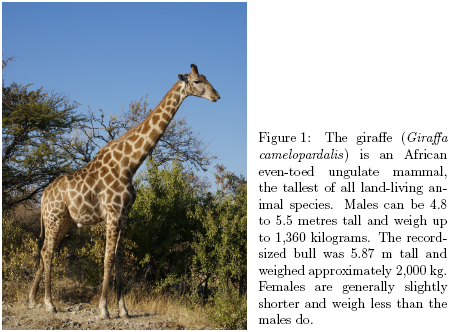
\includegraphics[width=0.48\textwidth]{./ingles/Latex_example_sidecap.jpg}
%  \end{center}
%\end{wrapfigure}

\begin{description}
\item[Nombre:] Born to be British
\item[Cristaleria:] Rock glass (6oz / 180cc)
\item[M\'etodo de elaboraci\'on:] Batido
\item[Decoraci\'on:] Rodajas de manzana
\end{description}

\begin{table}[h]
\caption{Ingredientes y proporciones} 
\label{tab:fonts}
\begin{center}       
\begin{tabular}{|l|l|l|c|l|} %% this creates two columns
%% |l|l| to left justify each column entry
%% |c|c| to center each column entry
%% use of \rule[]{}{} below opens up each row
\hline
\rule[-1ex]{0pt}{3.5ex}  \textbf{Producto} & \textbf{Bebida} & \textbf{Marca} & \textbf{Volumen} & \textbf{Fraccion}  \\
\hline
\rule[-1ex]{0pt}{3.5ex}  Aguardiente & Gin 			& Boodles British 		& 1  $\frac{1}{2}$ oz / 45 cc 	&  	\\
\hline
\rule[-1ex]{0pt}{3.5ex}  Licor 		& Triple Sec 	& Cointreau 				& $\frac{1}{4}$ oz / 7,5 cc 		&  	\\
\hline
\rule[-1ex]{0pt}{3.5ex}  Fruta 		& Manzana roja 	& Jugo	 				& 2 oz / 60 cc					& 	\\
\hline
\rule[-1ex]{0pt}{3.5ex}  Fruta 		& Manzana roja 	& Gajos (s/ c\'ascara)	& 4								& 	\\
\hline
\rule[-1ex]{0pt}{3.5ex}  Fruta 		& Manzana roja 	& Gajos chicos (s/ c\'ascara)	& 3								& 	\\
\hline
\rule[-1ex]{0pt}{3.5ex}  Fruta 		& lim\'on	 	& Gajos (s/ c\'ascara ni piel)	& 2								& 	\\
\hline
\rule[-1ex]{0pt}{3.5ex}  Jarabe		& Simple Syrup 	& 						& $\frac{3}{4}$ oz / 22,5 cc 		&  	\\
\hline
\end{tabular}
\end{center}
\end{table} 
Simple Syrup: 1 parte de agua y 1 parte de az\'ucar.
\bigskip 

%%-----------------------------------------------------------
\subsubsection{Formato de elaboraci\'on} 
\label{sec:title}
\bigskip 
\begin{center}
\begin{enumerate}
\item Colocar los gajos grandes de manzana y los de lim\'on en la coctelera.
\item Colocar el triple sec y el alm\'ibar en la coctelera.
\item Revolver estos ingredientes.
\item Agregar hielo en la coctelera.
\item Agregar el jugo de manzana y el gin.
\item Tapar la coctelera y batir.
\item Servir en vaso Rock Glass.
\item Decorar con los 3 gajos chicos de manzana. Dos pueden ir dentro del trago y el otro en el borde del vaso.
\end{enumerate}
\end{center}
\bigskip 
\bigskip 
%%%%%%%%%%%%%%%%%%%%%%%%%%%%%%%%%%%%%%%%%%%%%%%%%%%%%%%%%%%%%

\subsubsection{Notas}
\bigskip 
\begin{center}
\raggedright{}Servir sin sorbete.
\end{center} 

%\subsubsection{Informaci\'on extra}
\bigskip
%\begin{center}
\medskip 
%\raggedright{ \textbf{Or\'igenes de este trago}} \\ 
\medskip


%\end{center}
\newpage

\newpage
\bigskip \bigskip \bigskip
\subsection{Gin \& Tonic}
\bigskip 
\bigskip 
 
\subsubsection{Contenido}
\bigskip 
\begin{description}
\item[Nombre:] Gin \& Tonic
\item[Cristaleria:] Rock glass (6oz / 180cc)
\item[M\'etodo de elaboraci\'on:] Directo
\item[Decoraci\'on:] Rodajas de lima
\end{description}

\begin{table}[h]
\caption{Ingredientes y proporciones} 
\label{tab:fonts}
\begin{center}       
\begin{tabular}{|l|l|l|c|l|} %% this creates two columns
%% |l|l| to left justify each column entry
%% |c|c| to center each column entry
%% use of \rule[]{}{} below opens up each row
\hline
\rule[-1ex]{0pt}{3.5ex}  \textbf{Producto} & \textbf{Bebida} & \textbf{Marca} & \textbf{Volumen} & \textbf{Fraccion}  \\
\hline
\rule[-1ex]{0pt}{3.5ex}  Aguardiente & Gin 			& Boodles British 		& 2 oz / 60 cc 	&  	\\
\hline
\rule[-1ex]{0pt}{3.5ex}  Gaseosa		& Agua t\'onica 	& Schweppes 				& 4 oz / 120 cc 		&  	\\
\hline
\rule[-1ex]{0pt}{3.5ex}  Fruta 		& Lim\'on	 	& Exprimido				& $\frac{1}{2}$	lim\'on		& 	\\
\hline
\rule[-1ex]{0pt}{3.5ex}  Fruta 		& Lima		 	& 						& 1 rodaja		& 	\\
\hline
\end{tabular}
\end{center}
\end{table} 
\bigskip 

%%-----------------------------------------------------------
\subsubsection{Formato de elaboraci\'on} 
\label{sec:title}
\bigskip 
\begin{center}
\begin{enumerate}
\item Llenar un vaso Rock Glass con hielo.
\item Exprimir medio lim\'on en el vaso.
\item A\~nadir el gin y completar con el agua t\'onica.
\item Decorar con la rodaja de lima.
\end{enumerate}
\end{center}
\bigskip \bigskip 
\bigskip 
%%%%%%%%%%%%%%%%%%%%%%%%%%%%%%%%%%%%%%%%%%%%%%%%%%%%%%%%%%%%%

\subsubsection{Notas}
\bigskip 
\begin{center}
\raggedright{}Servir con sorbete.
\end{center} 
\bigskip \bigskip \bigskip 
\subsubsection{Informaci\'on extra}
\bigskip
\begin{center}

\medskip 
\raggedright{ \textbf{Or\'igenes de este trago}} \\ 
\medskip

{\justifying{
El origen del gin-tonic se sit\'ua en India, en el siglo XIX. Fue en la \'epoca, de expansi\'on territorial de Inglaterra. Durante su paso por India, donde predominaba la malaria, los colonos brit\'anicos tomaban quinina para evitar contagiarse. Preparaban una mezcla con quinina, agua y aromatizantes. M\'as tarde, Cadbury Schweppes (conocida hoy en d\'ia por sus bebidas gasificadas) sustituy\'o el agua por soda, para hacerla m\'as digerible, y crearon as\'i la ''Indian Water Tonic''. \\
\indent Para hacer la bebida m\'as rica, los soldados brit\'anicos, le a\~{n}adieron alcohol: la ginebra Bombay destilada en la ciudad del mismo nombre. As\'i nace el gin-tonic. En poco tiempo la mezcla pas\'o de ser una medicina preventiva a una bebida refrescante y social hasta el punto que en el a\~no 1870 la mezcla de Indian Water Tonic con ginebra era m\'as que conocida.\\ 
\indent Actualmente es una de las bebidas m\'as conocidas y consumidas del mundo y la podemos encontrar en cualquier bar al que vayamos.

La quinina es un alcaloide extra\'ido de la corteza del Quino. Es de sabor muy amargo con propiedades curativas. Anti\"{u}amente era utilizado para tratar la malaria, hasta que fue reemplazado por medicamentos sint\'eticos m\'as eficaces.
}\par}
\end{center}
\newpage
\end{document} 